{\color{teal!90}\chapter{Startup Issues with Launchers on Android}\label{cap:resetting}}

\AddToShipoutPictureBG*{%
  \AtPageUpperLeft{%
    \raisebox{-\height}{%
      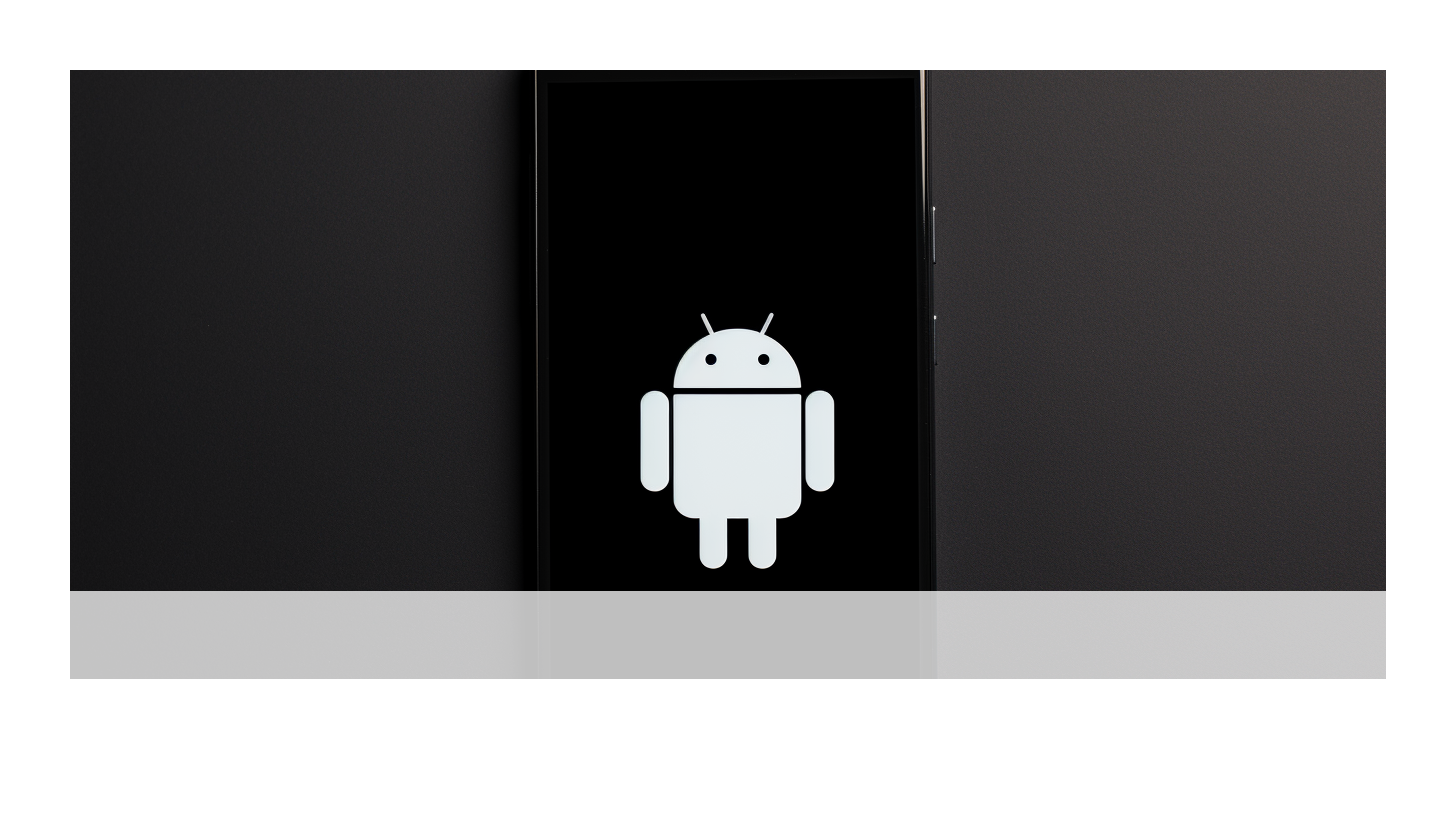
\includegraphics[width=\paperwidth]{./chapters/resetting-header.png}%
    }%
  }
}

\minitoc% Creating an actual minitoc mini lista contenuti

Installing a custom launcher on an Android device can sometimes lead to startup issues. In this chapter, we'll address how to handle a situation where the device doesn't boot properly after installing a custom launcher.

\section{The Problem}

After installing a custom launcher, difficulties booting up the device might arise. This could manifest as an infinite boot loop or an inability to access the user interface.

\section{The Solution}

To resolve this issue, follow these steps:

\begin{enumerate}
    \item Connect the Android device to your computer via Ethernet.
    \item Open a terminal window or command prompt on your computer.
    \item Use \cmd{adb connect \taishanIP }\footnote{\label{tv-ip} I've manually configured my device on \taishanIP \ so I won't need ARP or anything similar to discover the IP.} to verify that the device is recognized and connected properly.
    \item In the terminal, execute \cmd{adb reboot recovery} to reboot the device into recovery mode.
    \item Once the device is in recovery mode, use the remote controller to navigate and the OK button to select options.
    \item Select the \textbf{Wipe data/factory reset} option to erase all user data and application settings.
    \item After performing the data wipe, select the \textbf{Reboot system now} option to restart the device.
\end{enumerate}

It's important to note that selecting other options like \textbf{Reboot to bootloader} may lead to an endless boot loop. Therefore, it's advisable to avoid selecting these options unless you're experienced with recovery mode usage.




